\subsection{Diverse Interests}\label{sec:diversity}

The third alternative model we consider is a generalization of the altruistic model and the risk-averse model that we have discussed in previous sections. This class is characterized by diversity in the selfish behavior of its heterogeneous agents, in which agents pursue potentially different selfish goals (modeled by different individual user costs per agent).%, resulting in a routing solution of the whole network. 

Diverse selfish routing models are useful because they help us understand how we can leverage policies and natural diversity of goals in a network to increase the social welfare and efficiency of the network as a whole. For example, Beckmann et.al~\cite{beckmann1956studies} showed that tolls can help implement the social optimum at equilibrium when all agents have the same goal that is a linear combination of time and money.

However, there is some ambiguity in measuring the optimality of any outcome of the whole network with diverse selfish behavior. By definition, the objective function (what we regard as the social welfare cost) is different than from the single criterion in the case of selfish routing with agent homogeneity, where social welfare cost is equivalent to latency. Instead, there are multiple reasonable ways to characterize the social welfare of a diverse routing network. We will discuss the model adopted by Cole, Lianeas and Nikolova and their newly published results in 2018 \cite{ijcai2018-24}.

\subsubsection{Model}

We begin with same routing network with multiple source-destination pairs, using all our previous notations. However, there are now two criteria that the players consider in their individual user cost function.

Each agent wants to minimize their own cost $c^\omega$, which is a sum of two terms associated with two criteria. Let $\ell_P$ denote the cost of the first criterion (e.g., the latency) over some path $P=(s_i, t_i)$, and $\sigma_P$ be the cost of the second criterion, referred to as the {\it deviation function}. Then, given a routing $f$ of the network, the cost of that path is given by $c^\omega_p = \ell_P+\omega\cdot \sigma_P=\sum_{e\in P} \ell_e(f_e)+ \omega\sum_{e\in P}\sigma_e(f_e$), where $\omega$ is the {\it diversity parameter}. Each agent might have a different diversity parameter differentiating the degree to which they value the two criteria.

Note that the first criterion function (e.g., the latency function) has all the properties as we assumed in previous sections, while the deviation function $\sigma_e(x)$ is assumed to be continuous but not necessarily non-decreasing. However, the function $\ell_e+\omega\cdot \sigma_e$ must be non-decreasing. These assumptions are consistent with our previous risk-averse model in Section 3.2, because if $\sigma_e$ models the variance, then $\sigma_e$ could be decreasing in the flow.

Cole et. al. measures the effect of diversity on the resulting flow of a homogeneous agent population of the same size. The homogeneous agent population has the single diversity parameter $\bar{\omega}=\int \omega f(\omega)d r$. 

For a discrete distribution of $n$ discrete values $\omega_1^k, \dots, \omega_n^k$, the demand $d_k$ is a vector $d_k=(d_1^k, \dots, d_n^k)$ where each $d_i^k$ denotes the total demand of commodity $k$ with diversity parameter $\omega_i^k$. $d^k$ denotes commodity $k$'s total demand $d^k=\sum_{i=1}^n d_i^k$. For a heterogeneous equilibrium flow vector $g$, the {\it heterogeneous total cost} of commodity $k$ is denoted by $C^{k,ht}(g)=\sum_{j=1,\dots, n} d_j^k c^{k, \omega_j^k}(g)$, where $c^{k, \omega_j^k}(g)$ denotes the common cost at equilibrium $g$ for players of diversity parameter $\omega_j^k$ in commodity $k$. The heterogeneous total cost of $g$ is then $C^{ht}(g)=\sum_{k\in K} C^{k,ht}(g)$. 
%\XXX{Vibhaa: It might be helpful to give some intuition on how to think of these $r_i^k$ and $d_i^k$, like its not clear to me if the $n$ are the different agents in the graph and if so why would there be a different diversity parameter for every agent for every commodity. Even if that is the case, why does the demand vector have different components corresponding to the $n$ different diversity parameters? I'm pretty sure I'm misreading this, but I'm not sure how to interpret these variables is the high level  }

%Xiaoyue: each player has a diversity parameter. the same type of commodity can be sent by agent with different diversity parameters

For the corresponding homogeneous equilibrium flow $f$, i.e. the instance with diversity parameter $\bar{\omega}^k$, where $\bar{\omega}^k$ denotes the average diversity parameter for commodity $k$, players of commodity $k$ share the same cost $c^{\bar{\omega}^k}(f)$. In this case, the homogeneous total cost of commodity $k$ under $f$ is $C^{k,hm}(f)=d_kc^{\bar{\omega}^k}(f)$, and the homogeneous total cost of $f$ is $C^{hm}(f)=\sum_{k\in K} C^{k,hm}(f)$. 

\paragraph{Equilibrium flows} All equilibrium flows that we discuss for the diversity model are with respect to the {\it Wardrop equilibrium}. A flow $f$ is at the Wardrop equilibrium of an instance if for every $k\in K$, for every path $P\in \mathcal{P}_k$ with postive flow, and any diversity parameter $\omega$ on it, the path cost $c_P^\omega(f)\le c_{P'}^r(f)$ for all paths $P'\in \mathcal{P}_k$. It is known that a Nash equilibrium in a network game with a finite number of players converges to a Wardrop equilibrium in a network game with a finite number of players converges to a Wardrop equilibrium when the number of players increases \cite{haurie}.

\subsubsection{Results}
Let $g$ denote an equilibrium flow for the heterogeneous agent population and $f$ an equilibrium flow for the corresponding homogeneous agent population. Let $C^{ht}(g)$ denote the cost of flow $g$ and $C^{hm}(f)$ the cost of flow $f$. 

A {\it multi-commodity network} is consistent with all our previous models. We also introduce the definition of a {\it single-commodity network} as a network whose edges all belong to some single source-destination path as only these edges are going to be used by the equilibria and thus all other edges can be discarded. We present the following main results.

\begin{definition}
A directed $s-t$ network $G$ is {\it series-parallel} if it consists of a single edge $(s, t)$, or it is formed by the series or parallel composition of two series-parallel networks with terminals $(s_1, t_1)$ and $(s_2, t_2)$, respectively.
\end{definition}

The theorem below states that for single-commodity networks, diversity is always helpful in a single-commodity series parallel network.

\begin{theorem}
For any $s-t$ series-parallel network $G$ with a single commodity, we have $C^{ht}(g)\le C^{hm}(f)$.
\label{diverse1}
\end{theorem}

\begin{proof-sketch}

    The key observation is that since $f$ and $g$ route the same amount of flow from the unique source to the unique sink, there must be a path $P$ where $f$ sends no less flow along than $g$ does. Since the network is series-parallel, for every edge $e$ in $P$, $f_e \ge g_e$. This is true because a path in a series-parallel network can be broken up into some series-parallel parts in series and some series-parallel parts in parallel, which recursively breaks down to a simple series of edge(s). Hence for any $\omega\in [0, \omega_{\max}]$, we have $c_P^\omega (f)\ge c_P^\omega(g)$. We also know that $g$ could route more flow on $P$ but it doesn't, implying that there is no incentive for $g$ to switch the flow it sends on other paths to path $P$ under the same diversity parameter. Therefore $c^\omega(g)\le \sum_{e\in P} \ell_e(g_e)+\omega\sum_{e\in P}\sigma_e(g_e)$. Then $C^{ht}(g)\le \sum_{i=1}^k d_i(\sum_{e\in P} \ell_e(g_e)+\omega_i\sum_{e\in P}\sigma_e(g_e))=\ell_P(g)+\bar{\omega}\sigma_P(g)$ which is exactly the cost of the homogeneous equilibrium flow $f$ with the total demand being normalized to $1$ and the average diversity parameter is $\bar{\omega}=\sum_{i=1}^k d_i\omega_i$. Note that the last inequality wouldn't hold in the opposite direction. %Since $g$ is the heterogeneous equilibrium flow, which means that each agent is routing along the least cost route for itself, the cost of a unit flow $g$ is no larger than the cost of a unit of flow on $P$, while for $f$ the homogeneous equilibrium flow the agents all have the same cost as the cost of $f$ on $P$ per unit flow.
   %  \XXX{Vibhaa: This first made sense, but then I was wondering why the opposite isn't true, like why isn't there a path $P'$ where $g$ sends no less flow than $f$. Can't the opposite theorem also be proved?}  added explanation.
    %\XXX{Vibhaa: Does this denote the Nash equlibrium cost, if so make it clear?} Xiaoyue: added clarification in model.
    % \XXX{Vibhaa: not sure how the last part came come by, maybe I'm missing something trivial}.Xiaoyue: added clarification.
\end{proof-sketch}


\begin{theorem}
For any $s-t$ non-series-parallel network $G$ with a single commodity, there exists cost functions $C$ for which $C^{ht}(g)> C^{hm}(f)$.
\label{diversethm2}
\end{theorem}

\begin{proof-sketch}
    If $G$ is not series-parallel then the Braess graph (Figure~\ref{fig:braess}) can be embedded in it \cite{Valdes:1979:RSP:800135.804393}. Further, there are edge functions such that heterogeneous equilibrium flow has a larger cost than homogeneous equilibrium flow on a Braess graph. The deviation function $\sigma$ in such edge functions is $0$ on all edges other than the middle edge. Detailed examples can be found in \cite{ijcai2018-24}.
%The key reason is that for a series-parallel network, if two flows $|f|\ge |g|$, then there must be a parallel part $P_1$ of the network where $f$ sends more flow than $g$ on. This must be true because we can trivially think of the whole network as $P_1$. Since in a series-parallel network, we can decompose $P_1$ into some
%\XXX{Vibhaa: How does embedding a Braess graph help with this proof, might help to give some intuition}
\end{proof-sketch}

This theorem shows that diversity is always helpful in single-commodity networks if the network is series-parallel. Together with Theorem \ref{diverse1}, we know that the series-parallel structure is a necessary and sufficient condition for diversity to always be helpful.

Now we discuss our main results for multiple commodity networks. We use {\it average-respecting demand} to refer to the property that for any commodity $i,j: \bar{\omega}^i=\bar{\omega}^j$. 

A multi-commodity network $G$ can be decomposed in subnetworks $G_i$'s that each contains all the vertices and edges of $G$ that belong to a simple $s_i-t_i$ path for commodity $i$. WLOG, we assume these $G_i$ are acyclic.

\begin{definition}
    A multi-commodity network $G$ is {\it block-matching} if for every $i$, $G_i$ is series-parallel, and for every $i, j$, $G_i$ and $G_j$ are block-matching, respectively. %\XXX{Vibhaa: Can we use a picture or an example for this? series-parallel is fairly easy to visualize, but I'm not sure how to visualize this?}
\end{definition}


\begin{figure}{h}
  \begin{center}
    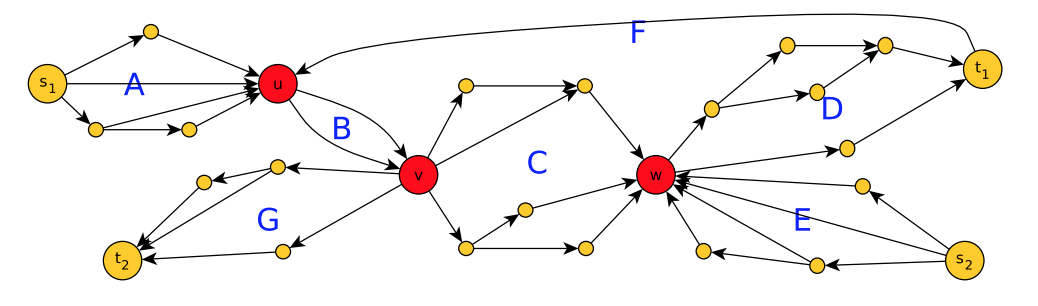
\includegraphics[width=0.8\textwidth]{block.png}
  \end{center}
  \caption{A block-matching network of $2$ commodities: $G_1=s_1 AuBvCwDt_1$ and $G_2=s_2EwDt_1FuBvGt_w$}
\end{figure}


The next theorem states that for multi-commodity networks, diversity is always helpful on any block-matching network with average-respecting demand. 

\begin{theorem}
For any $k$-commodity block-matching network with average-respecting demand, $C^{ht}(g)\le C^{hm}(f)$.
\label{diverse2}
\end{theorem}

\begin{proof-sketch}

Let's consider the block representation of a subnetwork $G_i=s_i B_1 v_1\dots v_{b_i-1} B _{b_i}t_i$ for some commodity $i$. Because $G$ is block-matching, for any block $B_j$ connecting $v_{j-1}$ and $v_j$ , any other commodity $j$ either contains block $B_j$ as a block in its block representation or contains none of the edges of $B_j$. This implies that under any routing of the demand, either all of $j$'s demand goes through $B_j$ or none of it does. So the total traffic routed by $f$ and $g$ are the same from $v_{j-1}$ to $v_j$. So if restricted to the block, the cost of the heterogeneous equilibrium is less than or equal to that of the homogeneous equilibrium by Theorem \ref{diverse1}; then the theorem is a result of summing over every block of all commodities.
%\XXX{Vibhaa: What are the $v_j$'s here and how do they relate to the block or how do we want to think about them (maybe I'm just still struggling to visualize this? Consequently, how do we go from traffic routed is the same on $f$ and $g$ to cost of heterogenous equlibrium being less than or equal to homogenous in a block} Xiaoyue: v_j are vertices. By previous theorem \ref{diverse1}.
\end{proof-sketch}



\begin{theorem}
For any $k$-commodity network, if diversity helps for every instance on $G$ with average-respecting demand, we have $C^{ht}(g)\le C^{hm}(f)$, then $G$ is a block-matching network.
\end{theorem}

\begin{proof-sketch}
    The proof is by contradiction. First, by our Theorem \ref{diversethm2} for single-commodity network, each subnetwork $G_i$ in our multi-commodity network must be a series-parallel network, otherwise we can use the same counterexample as for Theorem \ref{diversethm2}. Then since we can prove that any two commodities $i$ and $j$, any block of $G_i$ and any block of $G_j$ either have the same terminals and direction or their terminals has no intersection, we know that $G$ is block-matching. The detailed proof assumes the conditions does not hold, and then constructs demand and edge functions where diversity hurts to contradict the assumption. See \cite{ijcai2018-24}.
  % \XXX{Vibhaa: how can we prove this?}Xiaoyue: I think giving the main idea of the proofs is more important than repeating the whole proof in the paper.
\end{proof-sketch}

This theorem shows that diversity is always helpful in multi-commodity networks if the network is block-matching with average-respecting demand. Together with Theorem \ref{diverse2}, we know that the block-matching structure is a sufficient and necessary condition for diversity to always be helpful in a multi-commodity network.
